% TODO: 目前内容不足以凑满两页(正反 A4 纸),所以有些内容注释掉了,之后完善

\documentclass[UTF8]{article}
\setlength\parindent{0pt}
\pagenumbering{gobble}

\usepackage{geometry}
\geometry{papersize={210mm,297mm}}
\geometry{left=9mm,right=9mm,top=9mm,bottom=9mm}
\usepackage{fontspec}
\setmainfont{DejaVu Sans}[Scale=0.9]

\usepackage{xeCJK}
%\CJKfamily{zhsong} 由於 TeX Live 中自帶字體對於繁體中文字庫支援不佳,故註釋並改用其他字體
\setCJKmainfont[BoldFont=GenKiMin2TW-B.otf]{GenKiMin2TW-R.otf} %可在 ButTaiwan/genyo-font 取得
\setCJKsansfont[BoldFont=GenKiGothic2TW-B.otf]{GenKiGothic2TW-R.otf} %可在 ButTaiwan/genyog-font 取得

\usepackage{longfbox}
\usepackage{epstopdf}
\usepackage{float}
\usepackage{xpatch}
\usepackage{tipa}
\usepackage[export]{adjustbox}
\usepackage{enumitem}
\usepackage{mdframed}

\usepackage{multirow}
\usepackage{tabularx}
\renewcommand\tabularxcolumn[1]{m{#1}} % for vertical centering text in X column

\usepackage{multicol}
\usepackage[most]{tcolorbox}
\usepackage{amssymb}
\setlength{\columnsep}{3mm}

\usepackage[explicit,compact]{titlesec}
\titleformat{\section}{\normalfont\bfseries}{}{0pt}{【#1】}

% 啊!万能的 StackExchange!
% https://tex.stackexchange.com/questions/475466/latex-three-column-layout-merging-two-of-them-at-the-begining
%
\newlength{\abstractwidth}
\newlength{\columnshrink}
\newsavebox{\twocolinsert}
%
\makeatletter
\newlength{\resized@col}
\newcounter{column@count}
%
\xpatchcmd{\multi@column@out}{
	\process@cols\mult@firstbox{%
		\setbox\count@
		\vsplit\@cclv to\dimen@
		\set@keptmarks
		\setbox\count@
		\vbox to\dimen@
		{\unvbox\count@ \ifshr@nking\vfilmaxdepth\fi}%
	}%
}{
	\process@cols\mult@firstbox{%
		\global\advance\c@column@count\@ne
		\resized@col\dimen@%
		\ifnum\c@column@count=\tw@
				\advance\resized@col-\columnshrink
		\fi%
		\setbox\count@
		\vsplit\@cclv to\resized@col
		\set@keptmarks
		\setbox\count@
		\vbox to\dimen@{
			\ifnum
				\c@column@count=\tw@ \vspace*{\columnshrink}
			\fi
			\unvbox\count@
			\ifshr@nking\vfilmaxdepth\fi
		}%
	}%
}{\typeout{Success}}{\typeout{Failure}}
\makeatother

% for designing header
\newsavebox\mysavebox
\newenvironment{imgminipage}[2][]{%
   \def\imgcmd{\includegraphics[width=\wd\mysavebox, height=\dimexpr\ht\mysavebox+\dp\mysavebox\relax, #1]{#2}}%
   \begin{lrbox}{\mysavebox}%
   \begin{minipage}%
}{%
   \end{minipage}
   \end{lrbox}%
   \sbox\mysavebox{\setlength{\fboxrule}{0pt}\fbox{\usebox\mysavebox}}%
   \mbox{\rlap{\raisebox{-\dp\mysavebox}{\imgcmd}}\usebox\mysavebox}%
}

\renewcommand{\labelitemi}{$\blacktriangleright$}

\tcbset{
    frame code={}
    center title,
    left=0pt,
    right=0pt,
    top=6pt,
    bottom=0pt,
    colback=gray!40,
    colframe=white,
    enlarge left by=0mm,
    boxsep=0pt,
    arc=0pt,outer arc=0pt,
}

\begin{document}
\begin{multicols*}{3}

	\setlength{\abstractwidth}{2\linewidth}
	\addtolength{\abstractwidth}{\columnsep}
	\savebox{\twocolinsert}{\begin{minipage}{\abstractwidth}
		\setlength{\baselineskip}{13pt}
		\noindent 核准日期:2025年08月09日
		\newline 修改日期:2019年07月06日,2020年10月31日,2021年07月04日,
		\newline 2021年08月14日,2023年06月10日,2025年08月09日,
		\newline 2025年08月11日

		% \begin{mdframed}[leftline=false, rightline=false, innertopmargin=0pt, innerbottommargin=0pt, innerrightmargin=0pt, innerleftmargin=2em]
		% 	\includegraphics[width=0.15\abstractwidth, valign=m]{assets/debian-text.eps}
		% 	\hfill
		% 	\begin{imgminipage}{assets/header-background.eps}[t]{0.7\abstractwidth}
		% 		\Large \textbf{盒装安装媒介说明书}

		% 		\normalsize 请仔细阅读说明书并在管理员指导下使用
		% 	\end{imgminipage}
		% \end{mdframed}

		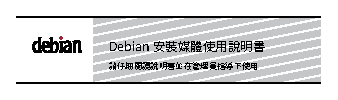
\includegraphics[width=\abstractwidth]{assets/header-zh-Hant.eps}


		\begin{mdframed}[hidealllines=true, innerbottommargin=.5em, innertopmargin=0pt]
			\sffamily

			{\centering 警告 \par}

			無論是否與其它作業系統合用,安裝 Debian 均存在遺失磁碟上所有內容的風險。(參見【不良反應】)

			某些與多媒體相關的軟體,特別是允許回放和提供音訊、影片操作或類似功能的軟體,不包含於 Debian,這是因為它在世界上的某些地區認定非法。本說明中的資訊和意見無意構成法律建議,法律意見可諮詢律師取得。

			一些硬體製造商拒絕告訴我們如何為他們的硬體編寫驅動程式。另一些則要求簽署不公開的合約才能接觸相關文件,以阻止我們發布驅動程式原始碼這項自由軟體的核心內容。因此這些硬體無法在 Linux 下運作。
		\end{mdframed}
	\end{minipage}}
	\setlength{\columnshrink}{\ht\twocolinsert}
	\addtolength{\columnshrink}{\dp\twocolinsert}
	\noindent\usebox{\twocolinsert}


	\begin{tcolorbox}
	\section*{發行版名稱}
	\end{tcolorbox}
	\begin{tabularx}{\linewidth}{@{}ll@{}}
		通用名稱: & Debian \\
		正式名稱: & Debian GNU/Linux \\
		英文讀音: & \textipa{["dEbi@n]} \\
	\end{tabularx}

	\medskip


	\begin{tcolorbox}
	\section*{內容}
	\end{tcolorbox}

	完全由自由軟體組成的類 UNIX 作業系統,其包含的多數軟體使用 GNU 通用公共授權協議授權,並由 Debian 計畫的參與者組成團隊打包、開發與維護。

	% 内核版本:4.19.0

	% 版本号:“buster”

	\medskip


	\begin{tcolorbox}
	\section*{性質}
	\end{tcolorbox}

	本系統為採用 GNU/Linux 內核的作業系統,安裝後可由 UEFI 或 Legacy 引導方式啟動。

	\medskip


	\begin{tcolorbox}
	\section*{適用平台}
	\end{tcolorbox}

	\begin{itemize}
		\item 可用於 arm64、amd64、i686、ppc64el、mipsel、s390x 等架構的電腦、伺服器和嵌入型裝置。
		\item 本包裝盒中的安裝媒體適用於何平台以實際為準。
	\end{itemize}


	\begin{tcolorbox}
	\section*{規格}
	\end{tcolorbox}

	1 枚 安裝媒體

	\medskip

	\begin{tcolorbox}
	\section*{用法}
	\end{tcolorbox}

	使用 USB 裝置引導。

	啟動方式依硬體調整,一般使用 UEFI。如有需要,亦可使用 Legacy。

	根據硬體效能和個人需要,調整安裝方式:一般而言,使用圖形化介面安裝;否則使用基於 ncurses 的指令列安裝程式。

	安裝基本系統並設定軟體套件後,即可視情況選擇桌面環境和視窗混成器。

	\medskip

	\begin{tcolorbox}
	\section*{不良反應}
	\end{tcolorbox}

	Debian 設有缺陷追蹤系統,用於歸檔管理使用者和開發者所提交的軟體缺陷報告,英文縮寫為 BTS。每個軟體缺陷報告都將授予一個編號並長期跟踪,直至標記為已修復。

	可在 https://www.debian.org/Bugs/ 獲取該檔案的複本。

	\medskip


	\begin{tcolorbox}
	\section*{注意事項}
	\end{tcolorbox}
	\begin{itemize}[leftmargin=*]

		\item 滿足運行的最低要求

		Pentium 4、1GHz 的處理器是桌上型系統的最低建議配置,下表是記憶體和硬碟的需求。

		{\small\begin{tabularx}{\linewidth}{|X|X|X|X|}
			\hline
			類別 & RAM\newline (最低) & RAM\newline (推薦) & 硬碟 \\
			\hline
			無桌面 & 128MB & 512MB & 2GB \\
			\hline
			有桌面 & 256MB & 1GB & 10GB \\
			\hline
		\end{tabularx}}

		基於您的需求,也許可以使用低於上表所列的配置完成系統安裝。但是多數用戶在無視這些建議的情況下會安裝失敗。

		\item 需要韌體的裝置

		除了需要裝置驅動程式,有些硬體還要在使用前載入韌體(firmware)或微碼(microcode)。

	\end{itemize}


	\begin{tcolorbox}
	\section*{禁忌}
	\end{tcolorbox}

	在使用中若出現或即將出現下列任何一種情況,請立即停止使用,並準備好系統恢復。

	\begin{itemize}[leftmargin=*]
		\setlength{\itemsep}{0pt}
		\setlength{\parskip}{0pt}
		\setlength{\parsep}{0pt}

		\item 以根權限在根目錄下執行遞迴刪除
		\item 未確認裝置代號即使用 dd 指令
		\item 未確認裝置代號即進行格式化
		\item 未確認操作即使用指令重新導向
		\item 未經確認即運行來自網路的指令集
		\item 長期在散熱不良的裝置上高負荷使用
	\end{itemize}


	 %\begin{tcolorbox}
	 %\section*{無障礙安裝}
	 %\end{tcolorbox}
	 
	 %Debian GNU/Linux 安裝媒體不用於視力或運動障礙人士。若確需安裝,請向管理員求助。

	 %\medskip

	 %\begin{tcolorbox}
	 %\section*{新手安裝}
	 %\end{tcolorbox}

	 %Debian GNU/Linux 應謹慎用於新手安裝,若需安裝,應由管理員全程指導,並持續監測系統運行,一旦系統完整度出現惡化,應考慮停止使用 Debian GNU/Linux。

	 %\medskip


	 %\begin{tcolorbox}
	 %\section*{版本迭代}
	 %\end{tcolorbox}
	 
	 %Debian 通常會按照一定的規律每隔一段時間發布一個新穩定版。Debian 穩定版本的生命週期為五年:首先是三年的完整支援,然後是兩年的長期支援(LTS)。
	 
	 %此外,在長期支援結束後,還有為期五年的擴充長期支援(ELTS),由三方服務商提供,且需支付一定費用。


	\begin{tcolorbox}
	\section*{系统相互作用}
	\end{tcolorbox}
	\begin{itemize}[leftmargin=*]
		\setlength{\parindent}{0pt}

		\item 與 Windows 的相互作用

		當您有雙重引導時,若另一個作業系統與 Windows 存取相同的檔案系統,這就有可能會導致問題與資料遺失。在這種情況下,檔案系統的真實狀態可能與 Windows 認為在「啟動」之後的情況不同,並且可能在進一步寫入檔案系統時導致檔案系統損毀。因此,為了避免檔案系統損毀,有必要在 Windows 中停用「快速啟動」功能。

		在罕見情況中已觀察到,在 Windows 進行系統更新時,可能會因重新啟動後 GRUB 引導被破壞,導致 Debian 無法啟動。同時,若在 Debian 安裝過程中將引導資訊寫入 Windows 所在的實體磁碟 MBR 內,將導致 Windows 無法正常啟動。

		\item 與其他 Linux 發行版的相互作用

		尚不明確。

	\end{itemize}


	\begin{tcolorbox}
	\section*{儲存}
	\end{tcolorbox}

	-40℃\textasciitilde +70℃

	妥善儲存所有安裝媒體,避免非技術人員接觸。

	\medskip


	\begin{tcolorbox}
	\section*{包裝}
	\end{tcolorbox}

	裝有 Debian GNU/Linux 安裝媒體的、支援 USB 3.0/2.0 協議的大容量存儲裝置。

	1 枚/盒

	\medskip


	\begin{tcolorbox}
	\section*{有效期}
	\end{tcolorbox}

	完整支援:36 个月

	長期支援:60 个月

	\medskip


	\begin{tcolorbox}
	\section*{執行標準}
	\end{tcolorbox}
	\begin{tabularx}{\linewidth}{@{}ll@{}}
		\multirow{4}{*}{}{開放原始碼許可:} & GNU GPL(主要)\\
		~ & GNU LGPL \\
		~ & BSD \\
		~ & 以及其他授權協議 \\
	\end{tabularx}

	\medskip


	\begin{tcolorbox}
	\section*{批准文號}
	\end{tcolorbox}

	說明書使用 CC-BY-SA 3.0 協議授權。

	\medskip


 	%\begin{tcolorbox}
 	%\section*{生產商}
  	%\end{tcolorbox}

	%Debian Project

	%\medskip


	\begin{tcolorbox}
	\section*{說明書}
	\end{tcolorbox}
	\begin{tabularx}{\linewidth}{@{}ll@{}}
		\multirow{2}{*}{}{編審:} & @YukariChiba\\
		~ & @moesoha \\
		~ & @pea-snow (繁體中文版)\\
		圖形: & @YJBeetle\\
		GitHub: & moesoha/debian-media-box\\
	\end{tabularx}

	\medskip


	\vfill
	\begin{flushright}
		Debian GNU/Linux - 13.0\linebreak 20250809
		\linebreak
		\newline
		\begin{minipage}{0,5\textwidth}
			\centering
			$\vcenter{\hbox{\includegraphics[height=10mm]{assets/debian-logo.eps}}}$
			$\vcenter{\hbox{\includegraphics[height=5mm]{assets/debian-text.eps}}}$
		\end{minipage}
	\end{flushright}

\end{multicols*}
\end{document}
